\chapter{Längenmetriken}

\section{Graphen --- Definitionen}

\begin{definition}{Graph}
  Ein \emph{Graph} $ G = (E, K) $ besteht aus einer \emph{Ecken}-Menge $ E $ und einer Menge von Paaren $ \{ u, v \} $ ($ u, v \in E $), genannt \emph{Kanten}.
\end{definition}

\begin{marginfigure}
    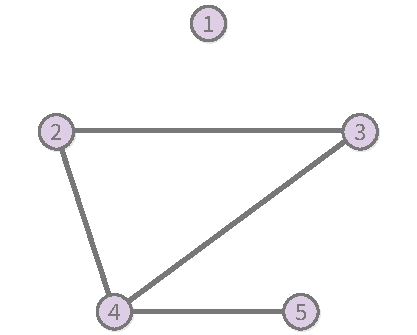
\includegraphics[width=\linewidth]{2017-10-18-03}
    \caption{Ein einfacher Graph. Dieser Graph ist \underline{nicht} zusammenhängend, da die Ecke $ 1 $ nicht von den anderen Ecken aus erreicht werden kann.}
\end{marginfigure}

\begin{definition}{Erreichbarkeit}
  Seien $ p, q \in E $ von $ G = (E, K) $. $ q $ ist \emph{erreichbar} von $ p $ aus, falls ein \emph{Kantenzug} von $ p $ nach $ q $ existiert.
\end{definition}

\begin{definition}{Zusammenhängend}
  $ G = (E, K) $ heißt \emph{zusammenhängend}, falls alle Ecken von einer beliebigen, festen Ecke aus erreichbar sind.
  \\ \ \\
  Ist $ G $ ein zusammenhängender Graph, so ist $ d(p, q) = $ minimale Kantenzahl eines Kantenzuges von $ p $ nach $ q $ eine Metrik.
\end{definition}

\begin{example}{Wortmetrik}
  Sei $ \Gamma \coloneqq \langle S \rangle $ vom endlichen Erzeugendensystem $ S $ erzeugte Gruppe. Dann:
  \begin{equation}
    \label{gl:wortmetrik}
    g \in \Gamma \Rightarrow g = s_1\cdot \dots s_n\text{ (multiplikativ, nicht eindeutig),}
  \end{equation}
  z.B. $ \Z = \langle \pm 1 \rangle $. \\
  Dann lässt sich über die Länge von $ g \in \Sigma $ (minimales $ n $ in \autoref{gl:wortmetrik}) eine Metrik definieren:
\end{example}

\begin{definition}{Wortmetrik}
  \begin{equation*}
    d_S(g, k) \coloneqq |g^{-1}k|
  \end{equation*}
  ist eine Metrik mit
  \begin{align*}
    d_s(kg,kh) &= |(kg)^{-1}kh| \\ 
    &= |g^{-1}\underbrace{k^{-1}k}_{=e}h| = |g^{-1}h| \\
    &= d_s(g,h)\text{,}
  \end{align*}
  also ist $ d_s $ linksmultiplikativ mit $ k \in \Gamma $ und damit eine Isometrie.
\end{definition}

\begin{definition}{Cayley-Graph}
  Der \emph{Cayley-Graph} $ \text{Cay}(\Gamma, S) $ von $ \Gamma $ bezüglich $ S $ ist der Graph $ G = (E, K) $ mit
  \begin{equation*}
    E \coloneqq \Gamma, \quad K \coloneqq \{ (g, gs) : g \in \Gamma, s \in S \}\text{.}
  \end{equation*}
  Die Graphen-Metrik auf $ \text{Cay}(\Sigma, S) $ ist isometrisch zur Wortmetrik.
\end{definition}

\begin{example}{Euklidische Metrik auf $ \R^2 $ als Standardmetrik}
  Sei
  \begin{equation*}
    c : [a,b] \to \R^2, \quad t \mapsto (x(t), y(t))
  \end{equation*}
  eine stückweise differenzierbare\sidenote{\textbf{Hinweis}: Mit \emph{differenzierbar} ist im Folgenden immer $ C^\infty $-differenzierbar gemeint, wenn nicht anders angegeben.} Kurve. \\
  Die \emph{euklidische Länge} von $ C $ ist
  \begin{align*}
    L_{\text{eukl}}(c) &\coloneqq \int_a^b \Vert C'(t) \Vert dt \quad \text{(via \emph{Polygon-Approximation})} \\
     &= \int_a^b \sqrt{\left( x'(t) \right)^2 + \left( y'(t) \right)^2}dt\text{.}
  \end{align*}
   \ \\
  \underline{Beispiel}: Geraden-Segment.
  \begin{equation*}
    g: [0,1] \to \R^2, \quad t \mapsto g(t) = (1-t)p + tq
  \end{equation*}
  Dann:
  \begin{equation*}
    g'(t) = -p+q, \quad \Vert g'(t) \Vert = \Vert p - q \Vert
  \end{equation*}
  und damit
  \begin{equation*}
    \underline{L_{\text{eukl}}(g)} = \int_0^1\Vert p - q \Vert dt = \Vert p - q \Vert = \underline{d_e(p,q)}\text{.}
  \end{equation*}
\end{example}

\begin{lemma}{Unabhängigkeit von $ \text{L}_\text{eukl} $}
  \label{lm:leuklinvarianz}
  \begin{enumerate}
    \item $ L_\text{eukl}(c) $ ist unabhängig von Kurvenparametrisierung.
    \item $ L_\text{eukl}(c) $ ist invariant unter Translationen, Drehungen und Spiegelungen.
  \end{enumerate}
  \begin{proof}
    \begin{enumerate}
      \item Zu zeigen: Für $ c: [a,b] \to \R^2 $, $ t \mapsto c(t) $ und einen monoton wachsenden Diffeomorphismus\sidenote{\textbf{Diffeomorphismus}: Bijektive, stetig differenzierbare Abbildung, deren Umkehrabbildung auch stetig differenzierbar ist.} $ t: [c, d] \to [a,b] $, $ s \mapsto t(s) $ gilt:
      \begin{equation*}
        L_\text{eukl}(c(t(s))) = L_\text{eukl}(c(t))\text{.}
      \end{equation*}
      Das folgt unmittelbar aus der Substitutionsregel für Integrale:
      \begin{equation*}
        \int_c^d \left\Vert \frac{dc}{ds} \right\Vert ds = \int_c^d \left\Vert \frac{d_c(t(s))}{dt} \right\Vert \frac{dt}{ds}ds = \int_{t(c) = a}^{t(d)=b} \left\Vert \frac{dc}{dt} \right\Vert dt \text{.}
      \end{equation*}\qed
      \item \begin{itemize}
        \item \underline{Translation}. \\ Für $ p = (p_1, \dots, p_n) \in \R^2 $ sei
        \begin{equation*}
           T_p(c(t)) = c(t) + p = (\lambda(t) + p_1, y(t) + p_2)
         \end{equation*} 
         die von $ p $ verschobene Kurve. Es gilt
         \begin{equation*}
           (T_p \circ c)(t) = c'(t) \Rightarrow \int_a^b \left\Vert (T_p \circ c)' \right\Vert dt = \int_a^b \left\Vert c' \right\Vert dt
         \end{equation*}
         und damit gilt das Lemma für Translationen. \qed
        \item \underline{Drehung}. \\
        Für $ \theta \in [0,2\pi] $ sei
        \begin{align*}
          D_\theta \circ c(t) &= \begin{pmatrix}
            \cos\theta & -\sin\theta \\
            \sin\theta & \cos\theta
          \end{pmatrix}c(t) \\ 
           &= (\cos\theta x(t) - \sin\theta y(t), \sin\theta x(t) + \cos\theta y(t))
        \end{align*}
        die um Winkel $ \theta $ gedrehte Kurve. \\
        Da $ D_\theta $ eine orthogonale Abbildung ist, folgt
        \begin{equation*}
          (D_\theta \circ c(t))' = D_\theta * c'(t)
        \end{equation*}
        und damit
        \begin{equation*}
          \left\Vert (D_\theta \circ c(t))' \right\Vert = \left\Vert D_\theta * c' \right\Vert \overset{\text{orth.}}{=} \left\Vert c' \right\Vert
        \end{equation*}
        und damit gilt das Lemma für Drehungen. \qed
        \item Spiegelungen sind wie Drehungen orthogonal, ihre Invarianz folgt aus der Invarianz der Drehungen.
      \end{itemize}
    \end{enumerate}
  \end{proof}
\end{lemma}

\begin{lemma}{Geraden sind am kürzesten}
  Die kürzesten Verbindungskurven zwischen Punkten in $ \R^2 $ sind genau die Geradensegmente. \\
  \begin{proof}
    Seien $ p, q \in \R^2 $ beliebig. Durch geeignete Rotation und Translation kann man $ (p,q) $ überführen in Punkte in spezieller Lage;
    \begin{equation*}
      p' = (0,0), \quad q' = (0,l)\text{.}
    \end{equation*}
    Wegen \autoref{lm:leuklinvarianz} ändert sich dabei die Länge entsprechender Verbindungskurven nicht. \\
    Sei jetzt $ c(t) \coloneqq (x(t),y(t)) $ eine stückweise differenzierbare Kurve zwischen $ p' $ und $ q' $. Dann gilt:
    \begin{align*}
      L_\text{eukl}(c) &= \int_a^b\sqrt{(x')^2+(y')^2}dt \geq \int_a^b\vert y' \vert dt \geq \int_a^by'(t)dt = \int_{y(a) = 0}^{y(b) = l} dy \\
       &= l\text{.}
    \end{align*}
    $ l $ ist die Länge des Geradensegmentes zwischen $ p' $ und $ q' $. \\
    $ \Rightarrow $ \underline{Infimum} der Längenwerte wird angenommen. Eindeutigkeit bleibt zu zeigen. \\
    Gilt für eine Kurve $ c $, dass $ L_\text{eukl}(c) = l $, so hat man in obigen Ungleichungen überall Gleichheit, also insbesondere $ x'(t) = 0 $ ($ \forall t $), also $ x(t) = \text{konstant} = x(0) = 0 $ und somit $ \widetilde{c} = (0,y(t)) $. Also ist $ \widetilde{c} $ auch (parametrisiertes) Geradensegment.
  \end{proof}
\end{lemma}

\begin{definition}{Euklidische Metrik auf $ \R^2 $-Kurven}
  Für $ p,q \in \R^2 $ sei $ \Omega_{pq}(\R^2) $ die Menge der stetig differenzierbaren Verbindungskurven zwischen $ p $ und $ q $. Wir setzen dann:
  \begin{equation*}
    (p,q) = \inf L_\text{eukl}(c), \quad c \in \Omega_{pq}(\R^2)\text{.}
  \end{equation*}
\end{definition}

\begin{theorem}{"Neuer" \ metrischer $ \R^2 $}
  \begin{equation*}
    (\R^2, d_\text{eukl})
  \end{equation*}
  ist ein metrischer Raum und isometrisch zu $ (\R^2, d_e) $.
\end{theorem}